\begin{center}
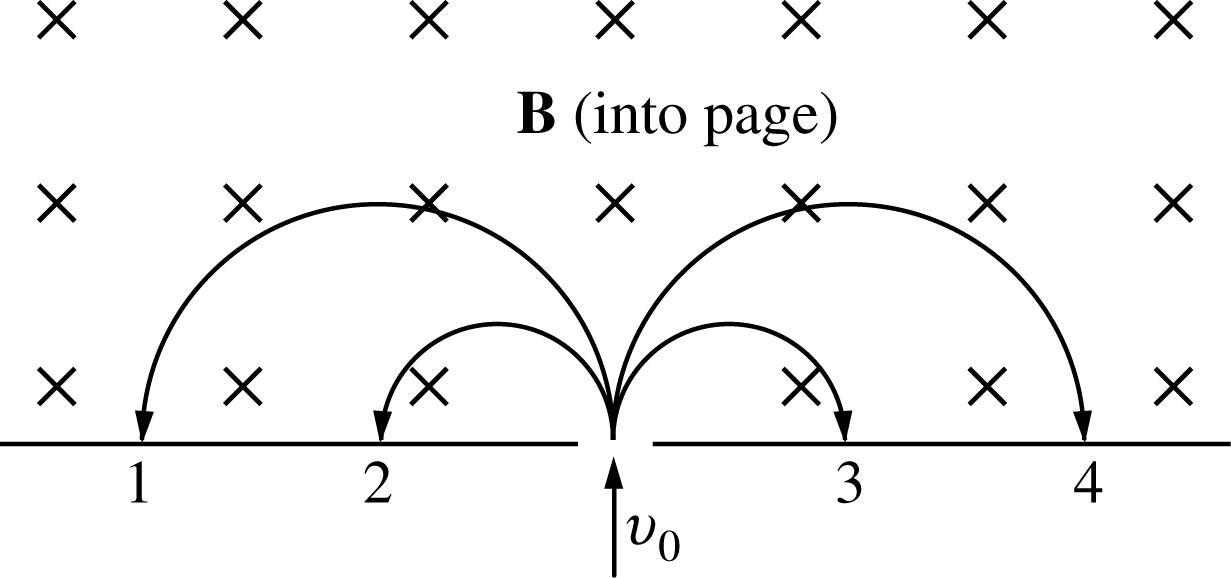
\includegraphics[scale=0.2]{images/img-004-003.png}
\end{center}

% Multiple Choice Question 5
\begin{questions}\setcounter{question}{4}\question
Two particles with the same speed $v_{0}$ enter a region of uniform magnetic field $\mathbf{B}$ directed into the page and are initially traveling perpendicular to $\mathbf{B}$, as shown above. Particle $Y$ has charge $-Q$ and mass $M$; particle $Z$ has charge $+Q$ and mass $2 M$. Which of the following pairs of paths shown is possible for the subsequent motion of the particles?

\tabto{0.75cm}{Particle $Y$}
\tabto{4.00cm}{Particle $Z$}\\
\tabto{0.75cm}\underline{$-Q, M$}
\tabto{4.00cm}\underline{$-Q, 2M$}

\begin{choices}
\choice 1 \tabto{3.25cm} 4
\choice 2 \tabto{3.25cm} 4
\choice 3 \tabto{3.25cm} 1
\choice 4 \tabto{3.25cm} 1
\choice 4 \tabto{3.25cm} 2
\end{choices}\end{questions}

